% !TeX spellcheck = en_US
\section{Experiments}\label{sec:experiments}
In this section, we present the results of all the experiments described before in this document.  

All the evaluations are performed using Set5 \cite{SET5} and Set14 \cite{SET14}, which are degraded by applying the following algorithms in order to obtain the \gls{lr} images:

\begin{itemize}
\item First, all the images in Set5 and Set14 are downscaled using Lanczos interpolation with a scale factor of 2. 
\item Second, we apply one of the following noise types varying the noise parameters in order to enlarge the test set:
\begin{itemize}
	\item Gaussian noise is applied using $\mu=0$ and $\sigma = 0.05, \sigma = 0.10$ and $\sigma = 0.15$.
	\item Poisson noise is applied using input pixels values as means of Poisson distributions scaled up by $2^8$.
	\item Salt-and-pepper and uniform noise is applied using noise ratios of $0.05, 0.10, 0.15$ and $0.20$.
\end{itemize}
\end{itemize}

After applying these filters with their respective parameter variations, we end up having 12 sets of 19 images, making a total of 228 \gls{lr} images, which correspond to the 19 \gls{hr} images of Set5 and Set14. Figure \ref{fig:exp0} shows some examples of this processing applied to the ``baby'' image from Set5.

\begin{figure}
	\centering
	\begin{subfigure}{0.24\textwidth}
		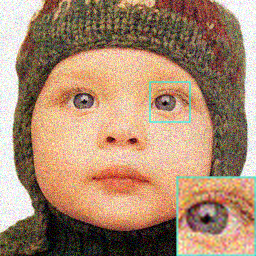
\includegraphics[width=\textwidth]{images/exp0.1/gaussian0.png}
		\caption{Gaussian, $\sigma=0.1$}
	\end{subfigure}
	\begin{subfigure}{0.24\textwidth}
		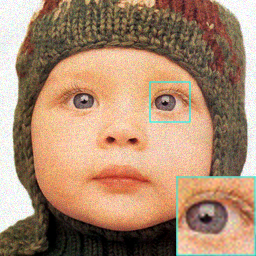
\includegraphics[width=\textwidth]{images/exp0.1/poisson0.png}
		\caption{Poisson}
	\end{subfigure}
	\begin{subfigure}{0.24\textwidth}
		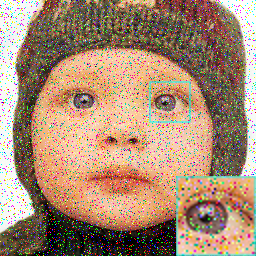
\includegraphics[width=\textwidth]{images/exp0.1/salt0.png}
		\caption{S\&P, $r=0.1$}
	\end{subfigure}
	\begin{subfigure}{0.24\textwidth}
		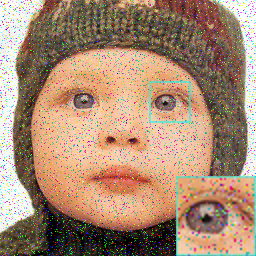
\includegraphics[width=\textwidth]{images/exp0.1/uniform0.png}
		\caption{Uniform, $r=0.1$}
	\end{subfigure}
\caption{The image ``baby'' from Set5, degraded using downscaling with a factor of 2 and different types of noise.}
\label{fig:exp0}
\end{figure}

The same 228 images are used for all the experiments. All the settings can be found along with the implementation of the \glspl{cnn} and the datasets. 

For the experiments that make use of median filter and wavelet denoiser, we apply the \textsc{matlab} functions \texttt{medfilt2()} and \texttt{wdenoise2()}.

In order to perform the evaluation of the quality metrics, the \textsc{matlab} functions \texttt{psnr()} and \texttt{ssim()} are used.

\subsection{Experiment 1.1}
In this experiment, we evaluate \gls{fsrcnn} $+$ \gls{ircnn} on our set of 228 \gls{lr} images. The results of this experiment are presented in Table \ref{tab:experiment11}.

\begin{table}[h]
	\centering
	\begin{tabular}{|l|l|r|r|r|r|}
		\hline
		\rowcolor[HTML]{EFEFEF} 
		\multicolumn{1}{|c|}{\cellcolor[HTML]{EFEFEF}\textbf{Noise}} & \textbf{Parameters} & \multicolumn{1}{c|}{\cellcolor[HTML]{EFEFEF}\textbf{Set5 \gls{psnr} (dB)}} & \multicolumn{1}{c|}{\cellcolor[HTML]{EFEFEF}\textbf{Set5 \gls{ssim}}} & \multicolumn{1}{c|}{\cellcolor[HTML]{EFEFEF}\textbf{Set14 \gls{psnr} (dB)}} & \multicolumn{1}{c|}{\cellcolor[HTML]{EFEFEF}\textbf{Set14 \gls{ssim}}} \\ \hline
		\rowcolor[HTML]{FFFFFF} 
		\cellcolor[HTML]{EFEFEF} & $\mu=0, \sigma=0.05$ & 26.6621 & 0.8639 & 25.1018 & 0.8065 \\
		\rowcolor[HTML]{EFEFEF} 
		\cellcolor[HTML]{EFEFEF} & $\mu=0, \sigma=0.10$ & 21.5502 & 0.7024 & 20.6851 & 0.6294 \\
		\rowcolor[HTML]{FFFFFF} 
		\multirow{-3}{*}{\cellcolor[HTML]{EFEFEF}Gaussian} & $\mu=0, \sigma=0.15$ & 18.4371 & 0.5669 & 17.7753 & 0.4954 \\
		\rowcolor[HTML]{EFEFEF} 
		Poisson & $peak=2^8$ & 27.9000 & 0.9074 & 25.9664 & 0.8401 \\
		\rowcolor[HTML]{FFFFFF} 
		\cellcolor[HTML]{EFEFEF} & $r=0.05$ & 22.1321 & 0.7678 & 21.1879 & 0.6994 \\
		\rowcolor[HTML]{EFEFEF} 
		\cellcolor[HTML]{EFEFEF} & $r=0.10$ & 18.6522 & 0.6218 & 18.0292 & 0.5487 \\
		\rowcolor[HTML]{FFFFFF} 
		\cellcolor[HTML]{EFEFEF} & $r=0.15$ & 16.4730 & 0.5141 & 16.0007 & 0.4431 \\
		\rowcolor[HTML]{EFEFEF} 
		\multirow{-4}{*}{\cellcolor[HTML]{EFEFEF}Salt-and-pepper} & $r=0.20$ & 14.9244 & 0.4320 & 14.5495 & 0.3670 \\
		\rowcolor[HTML]{FFFFFF} 
		\cellcolor[HTML]{EFEFEF} & $r=0.05$ & 24.3520 & 0.8135 & 23.4238 & 0.7688 \\
		\rowcolor[HTML]{EFEFEF} 
		\cellcolor[HTML]{EFEFEF} & $r=0.10$ & 20.9578 & 0.7032 & 20.5673 & 0.6542 \\
		\rowcolor[HTML]{FFFFFF} 
		\cellcolor[HTML]{EFEFEF} & $r=0.15$ & 18.7674 & 0.6155 & 18.6073 & 0.5642 \\
		\rowcolor[HTML]{EFEFEF} 
		\multirow{-4}{*}{\cellcolor[HTML]{EFEFEF}Uniform} & $r=0.20$ & 17.1090 & 0.5410 & 17.1459 & 0.4914 \\
		\rowcolor[HTML]{FFFFFF} 
		\textbf{All} &  & \textbf{20.6598} & \textbf{0.6708} & \textbf{19.9200} & \textbf{0.6090}\\\hline
	\end{tabular}
	\caption{\gls{psnr} and \gls{ssim} results for the Experiment 1.1}
	\label{tab:experiment11}
\end{table}

In the table, we can see quite low values of \gls{psnr} and \gls{ssim} for both Set5 and Set14. In fact, if we visually inspect the results, we can observe that the images present a large amount of noise for all the cases. This is shown in Figure \ref{fig:exp1.1}, that exposes the results of restoring the downscale, noisy images of Figure \ref{fig:exp0} using \gls{fsrcnn} $+$ \gls{ircnn}.

\begin{figure}
	\centering
	\begin{subfigure}{0.24\textwidth}
		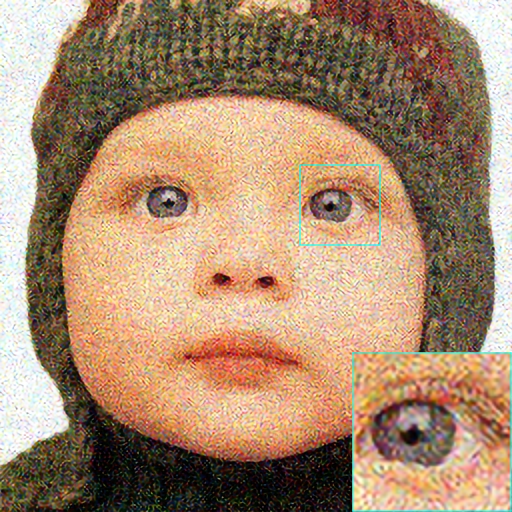
\includegraphics[width=\textwidth]{images/exp1.1/gaussian.png}
		\caption{Gaussian restored}
	\end{subfigure}
	\begin{subfigure}{0.24\textwidth}
		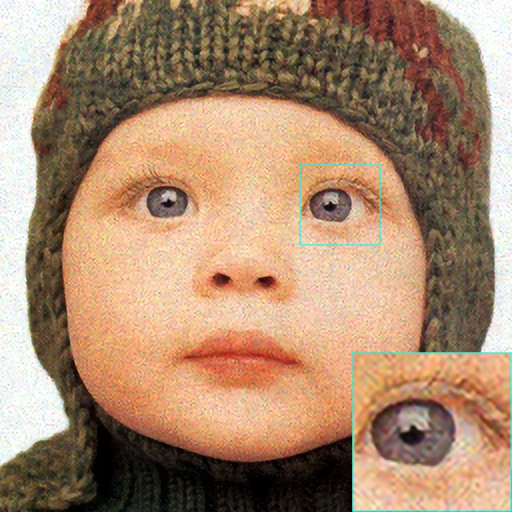
\includegraphics[width=\textwidth]{images/exp1.1/poisson.png}
		\caption{Poisson restored}
	\end{subfigure}
	\begin{subfigure}{0.24\textwidth}
		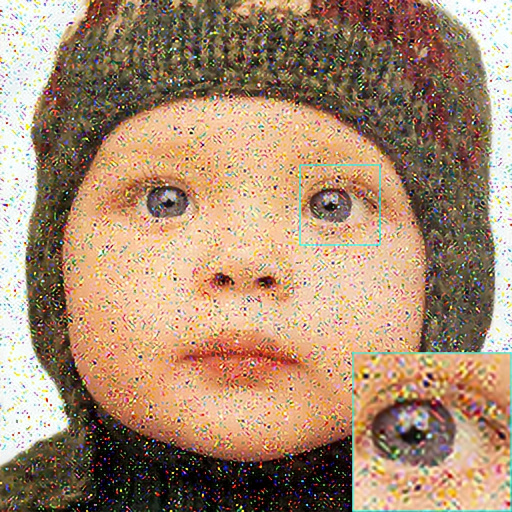
\includegraphics[width=\textwidth]{images/exp1.1/salt.png}
		\caption{S\&P restored}
	\end{subfigure}
	\begin{subfigure}{0.24\textwidth}
		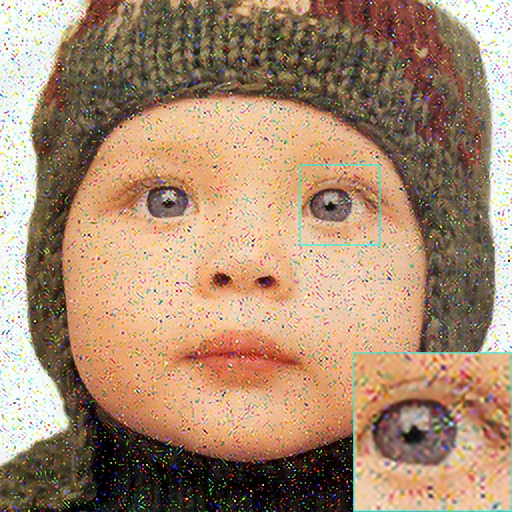
\includegraphics[width=\textwidth]{images/exp1.1/uniform.png}
		\caption{Uniform restored}
	\end{subfigure}
	\caption{Experiment 1.1: restoration using \gls{fsrcnn} $+$ \gls{ircnn}}
	\label{fig:exp1.1}
\end{figure}

In the figure, we can see that applying the networks in this order cannot remove the noise of the images properly. Instead, \gls{fsrcnn} tries to super-resolve the noise pixels, mixing up the good information of the image with them. Once the image is super-resolved, \gls{ircnn} tries to remove the noise. However, in this case, the resulting noise is a super-resolved version of the original applied noise, and therefore, the network is not capable of detecting the residual part of the image.

This effect repeats for all the images in both Set5 and Set14 and for all noise types. As a consequence, we can observe low \gls{psnr} and \gls{ssim} values in Table \ref{tab:experiment11}.

The results of this experiment shows us that \gls{fsrcnn} $+$ \gls{ircnn} will produce low quality results and that it is not appropriate to super-resolve and denoise our \gls{lr} images.

\subsection{Experiment 1.2}
In this experiment, we reverse the order of the networks from the previous experiment and evaluate instead the results of applying \gls{ircnn} $+$ \gls{fsrcnn} to our set of \gls{lr} images. Table \ref{tab:experiment12} shows the quality metrics results for this experiment. 

\begin{table}[]
	\centering
	\begin{tabular}{|l|l|r|r|r|r|}
		\hline
		\rowcolor[HTML]{EFEFEF} 
		\multicolumn{1}{|c|}{\cellcolor[HTML]{EFEFEF}\textbf{Noise}} & \textbf{Parameters} & \multicolumn{1}{c|}{\cellcolor[HTML]{EFEFEF}\textbf{Set5 \gls{psnr}}} & \multicolumn{1}{c|}{\cellcolor[HTML]{EFEFEF}\textbf{Set5 \gls{ssim}}} & \multicolumn{1}{c|}{\cellcolor[HTML]{EFEFEF}\textbf{Set14 \gls{psnr} (dB)}} & \multicolumn{1}{c|}{\cellcolor[HTML]{EFEFEF}\textbf{Set14 \gls{ssim}}} \\ \hline
		\rowcolor[HTML]{FFFFFF} 
		\cellcolor[HTML]{EFEFEF} & $\mu=0, \sigma=0.05$ & 29.4125 & 0.9055 & 27.1441 & 0.8704 \\
		\rowcolor[HTML]{EFEFEF} 
		\cellcolor[HTML]{EFEFEF} & $\mu=0, \sigma=0.10$ & 27.3907 & 0.8825 & 25.6060 & 0.8255 \\
		\rowcolor[HTML]{FFFFFF} 
		\multirow{-3}{*}{\cellcolor[HTML]{EFEFEF}Gaussian} & $\mu=0, \sigma=0.15$ & 26.0656 & 0.8709 & 24.4851 & 0.7896 \\
		\rowcolor[HTML]{EFEFEF} 
		Poisson & $peak=2^8$ & 30.1634 & 0.9314 & 27.5250 & 0.8855 \\
		\rowcolor[HTML]{FFFFFF} 
		\cellcolor[HTML]{EFEFEF} & $r=0.05$ & 32.3303 & 0.9585 & 28.8342 & 0.9176 \\
		\rowcolor[HTML]{EFEFEF} 
		\cellcolor[HTML]{EFEFEF} & $r=0.10$ & 31.8659 & 0.9498 & 28.5673 & 0.9119 \\
		\rowcolor[HTML]{FFFFFF} 
		\cellcolor[HTML]{EFEFEF} & $r=0.15$ & 31.3457 & 0.9453 & 28.2604 & 0.9067 \\
		\rowcolor[HTML]{EFEFEF} 
		\multirow{-4}{*}{\cellcolor[HTML]{EFEFEF}Salt-and-pepper} & $r=0.20$ & 30.6621 & 0.9395 & 27.8548 & 0.8990 \\
		\rowcolor[HTML]{FFFFFF} 
		\cellcolor[HTML]{EFEFEF} & $r=0.05$ & 32.2225 & 0.9559 & 28.7999 & 0.9160 \\
		\rowcolor[HTML]{EFEFEF} 
		\cellcolor[HTML]{EFEFEF} & $r=0.10$ & 31.5749 & 0.9459 & 28.4277 & 0.9089 \\
		\rowcolor[HTML]{FFFFFF} 
		\cellcolor[HTML]{EFEFEF} & $r=0.15$ & 30.8047 & 0.9390 & 27.9306 & 0.8999 \\
		\rowcolor[HTML]{EFEFEF} 
		\multirow{-4}{*}{\cellcolor[HTML]{EFEFEF}Uniform} & $r=0.20$ & 29.8574 & 0.9319 & 27.2938 & 0.8875 \\
		\rowcolor[HTML]{FFFFFF} 
		\textbf{All} &  & \textbf{30.3080} & \textbf{0.9297} & \textbf{27.5607} & \textbf{0.8849}\\\hline
	\end{tabular}
	\caption{\gls{psnr} and \gls{ssim} results for the Experiment 1.2}
	\label{tab:experiment12}
\end{table}

First of all, we can see a \gls{psnr} value of $30.3080dB$ on the images of Set5 and $27.5697dB$ on the images of Set14, which improves the results of the previous experiment by $+8.6489dB$ in average. On the other hand, the \gls{ssim} results in this case are $0.9297$ and $0.8849$, which are much closer to $1$ than the values obtained in Experiment 1.1.

This improvement on the metrics can be also observed in Figure \ref{fig:exp1.2}, in which we present the results of applying \gls{ircnn} $+$ \gls{fsrcnn} on the images of Figure \ref{fig:exp0}. By reversing the order of the networks, we can see that the images get denoised and super-resolved, not presenting large amounts of noise as seen in the results of Experiment 1.1.

\begin{figure}
	\centering
	\begin{subfigure}{0.24\textwidth}
		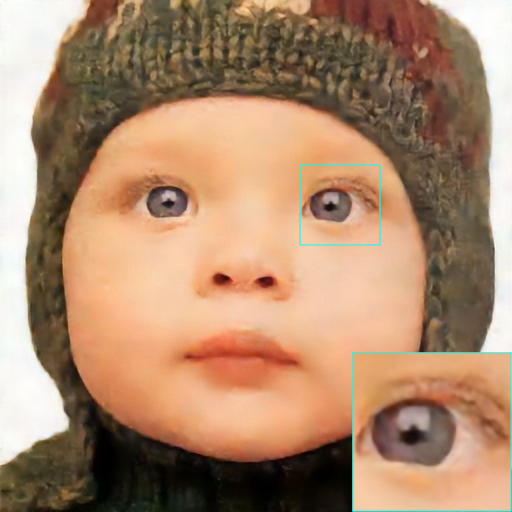
\includegraphics[width=\textwidth]{images/exp1.2/gaussian.png}
		\caption{Gaussian restored}
	\end{subfigure}
	\begin{subfigure}{0.24\textwidth}
		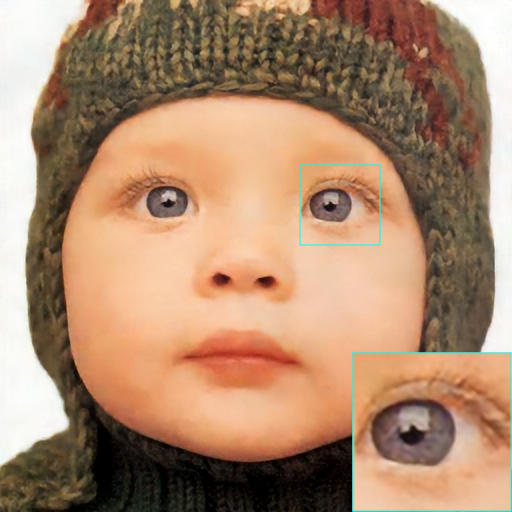
\includegraphics[width=\textwidth]{images/exp1.2/poisson.png}
		\caption{Poisson restored}
	\end{subfigure}
	\begin{subfigure}{0.24\textwidth}
		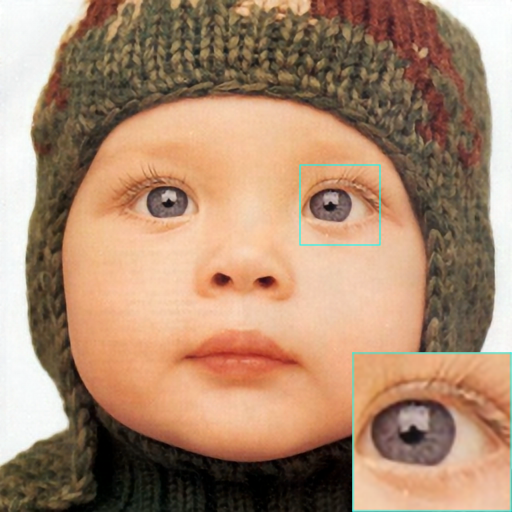
\includegraphics[width=\textwidth]{images/exp1.2/salt.png}
		\caption{S\&P restored}
	\end{subfigure}
	\begin{subfigure}{0.24\textwidth}
		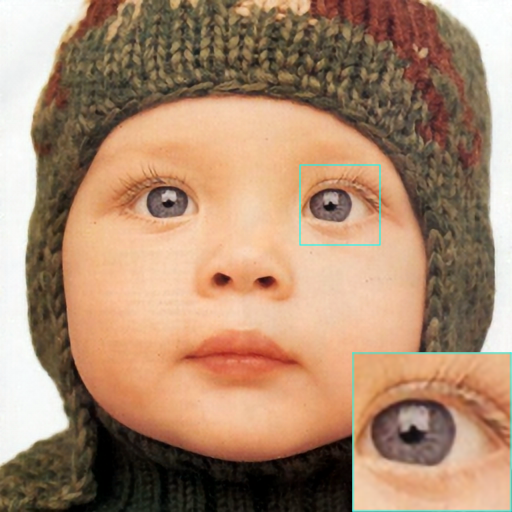
\includegraphics[width=\textwidth]{images/exp1.2/uniform.png}
		\caption{Uniform restored}
	\end{subfigure}
	\caption{Experiment 1.2: restoration using \gls{ircnn} $+$ \gls{fsrcnn}}
	\label{fig:exp1.2}
\end{figure}

In this case, \gls{ircnn} first removes the residual, obtaining an approximation to the downscale version of the \gls{hr} image. Once this is done, \gls{fsrcnn} super-resolves the denoised output in order to obtain the \gls{hr} image. 

Given these results, the next sets of experiments, which use both traditional and deep learning based methods, apply the algorithms following this logical order: the corresponding denoiser is applied (\gls{ircnn}, wavelet denoiser or median filter) followed by the \gls{sisr} algorithm (\gls{fsrcnn} or bicubic interpolation).


\subsection{Experiment 2.1}

In this experiment, we evaluate the results of replacing \gls{fsrcnn} by bicubic interpolation in the previous experiment. By doing this, we intend to analyze how a traditional method performs in comparison to a deep learning method when combined with \gls{ircnn}. The results of this experiment are exposed in Table \ref{tab:experiment21}.

\begin{table}[]
	\centering
	\begin{tabular}{|l|l|r|r|r|r|}
		\hline
		\rowcolor[HTML]{EFEFEF} 
		\multicolumn{1}{|c|}{\cellcolor[HTML]{EFEFEF}\textbf{Noise}} & \textbf{Parameters} & \multicolumn{1}{c|}{\cellcolor[HTML]{EFEFEF}\textbf{Set5 \gls{psnr}}} & \multicolumn{1}{c|}{\cellcolor[HTML]{EFEFEF}\textbf{Set5 \gls{ssim}}} & \multicolumn{1}{c|}{\cellcolor[HTML]{EFEFEF}\textbf{Set14 \gls{psnr} (dB)}} & \multicolumn{1}{c|}{\cellcolor[HTML]{EFEFEF}\textbf{Set14 \gls{ssim}}} \\ \hline
		\rowcolor[HTML]{FFFFFF} 
		\cellcolor[HTML]{EFEFEF} & $\mu=0, \sigma=0.05$ & 29.1069 & 0.9188 & 26.7379 & 0.8608 \\
		\rowcolor[HTML]{EFEFEF} 
		\cellcolor[HTML]{EFEFEF} & $\mu=0, \sigma=0.10$ & 27.3585 & 0.8963 & 25.4602 & 0.8206 \\
		\rowcolor[HTML]{FFFFFF} 
		\multirow{-3}{*}{\cellcolor[HTML]{EFEFEF}Gaussian} & $\mu=0, \sigma=0.15$ & 26.1240 & 0.8824 & 24.4524 & 0.7874 \\
		\rowcolor[HTML]{EFEFEF} 
		Poisson & $peak=2^8$ & 29.7801 & 0.9419 & 27.0475 & 0.8742 \\
		\rowcolor[HTML]{FFFFFF} 
		\cellcolor[HTML]{EFEFEF} & $r=0.05$ & 31.2225 & 0.9585 & 27.9022 & 0.8994 \\
		\rowcolor[HTML]{EFEFEF} 
		\cellcolor[HTML]{EFEFEF} & $r=0.10$ & 30.9084 & 0.9538 & 27.7169 & 0.8953 \\
		\rowcolor[HTML]{FFFFFF} 
		\cellcolor[HTML]{EFEFEF} & $r=0.15$ & 30.5699 & 0.9503 & 27.5133 & 0.8908 \\
		\rowcolor[HTML]{EFEFEF} 
		\multirow{-4}{*}{\cellcolor[HTML]{EFEFEF}Salt-and-pepper} & $r=0.20$ & 30.1156 & 0.9454 & 27.2382 & 0.8842 \\
		\rowcolor[HTML]{FFFFFF} 
		\cellcolor[HTML]{EFEFEF} & $r=0.05$ & 31.1893 & 0.9577 & 27.8885 & 0.8988 \\
		\rowcolor[HTML]{EFEFEF} 
		\cellcolor[HTML]{EFEFEF} & $r=0.10$ & 30.7560 & 0.9519 & 27.6282 & 0.8933 \\
		\rowcolor[HTML]{FFFFFF} 
		\cellcolor[HTML]{EFEFEF} & $r=0.15$ & 30.2349 & 0.9463 & 27.2898 & 0.8858 \\
		\rowcolor[HTML]{EFEFEF} 
		\multirow{-4}{*}{\cellcolor[HTML]{EFEFEF}Uniform} & $r=0.20$ & 29.5822 & 0.9393 & 26.8459 & 0.8753 \\
		\rowcolor[HTML]{FFFFFF} 
		\textbf{All} &  & \textbf{29.7457} & \textbf{0.9369} & \textbf{26.9767} & \textbf{0.8722}\\\hline
	\end{tabular}
	\caption{\gls{psnr} and \gls{ssim} results for the Experiment 2.1}
	\label{tab:experiment21}
\end{table}

In the table, we can see that, in average, the overall \gls{psnr} and \gls{ssim} results are $0.5732dB$ and $0.0028$ units lower than the results of Experiment 1.2, respectively. However, if we take a look at the \gls{ssim} results on the five images of Set5, we see a slight improvement when we choose bicubic interpolation over \gls{fsrcnn}.

In Figure \ref{fig:exp2.1} we present the results of applying \gls{ircnn} $+$ bicubic interpolation to the images of \ref{fig:exp0}. In this case, we can see that the bicubic interpolation provides good results as well, however it cannot conserve the image edges as well as \gls{fsrcnn} does when super-resolving the \gls{lr} images.

\begin{figure}
	\centering
	\begin{subfigure}{0.24\textwidth}
		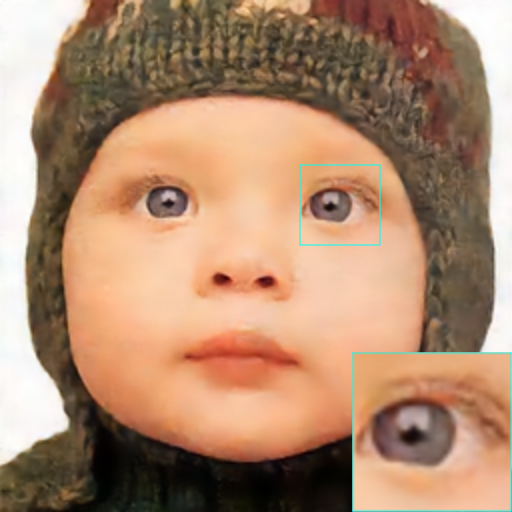
\includegraphics[width=\textwidth]{images/exp2.1/gaussian.png}
		\caption{Gaussian restored}
	\end{subfigure}
	\begin{subfigure}{0.24\textwidth}
		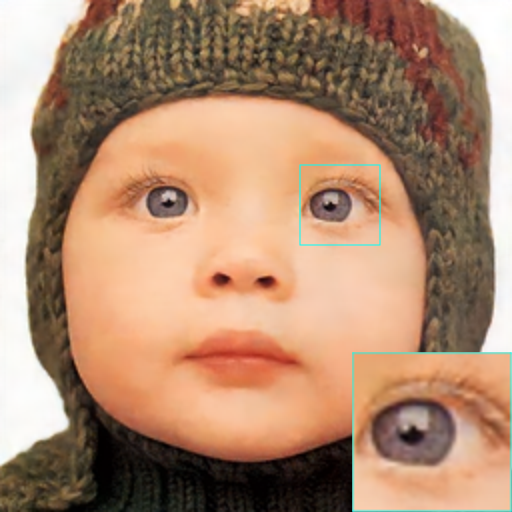
\includegraphics[width=\textwidth]{images/exp2.1/poisson.png}
		\caption{Poisson restored}
	\end{subfigure}
	\begin{subfigure}{0.24\textwidth}
		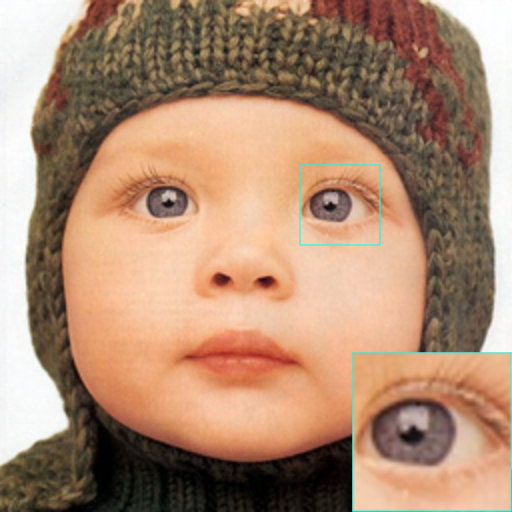
\includegraphics[width=\textwidth]{images/exp2.1/salt.png}
		\caption{S\&P restored}
	\end{subfigure}
	\begin{subfigure}{0.24\textwidth}
		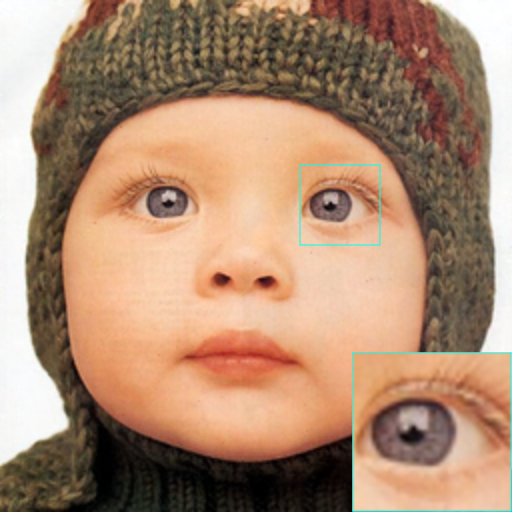
\includegraphics[width=\textwidth]{images/exp2.1/uniform.png}
		\caption{Uniform restored}
	\end{subfigure}
	\caption{Experiment 2.1: restoration using \gls{ircnn} $+$ bicubic interpolation}
	\label{fig:exp2.1}
\end{figure}

This results show that even though in average \gls{fsrcnn} performs better, there might be some cases in which the bicubic interpolation approximates better the original \gls{hr} image.

However, the performance of the \gls{sisr} algorithms is being compared using the output of \gls{ircnn} as an input, which is the result of convolving the noisy \gls{lr} image with the corresponding \gls{ircnn} filters. Hence, even though the \gls{ssim} results for Set5 show better performance for bicubic interpolation, we show in Table \ref{tab:experiment} that \gls{fsrcnn} overperforms bicubic interpolation if we use the downscaled images without noise as the input of both algorithms.

\begin{table}[]
	\centering
	\begin{tabular}{|l|r|r|r|r|}
		\hline
		\rowcolor[HTML]{EFEFEF}
		\multicolumn{1}{|c}{\cellcolor[HTML]{EFEFEF}\textbf{Method}} &
		\multicolumn{1}{c|}{\cellcolor[HTML]{EFEFEF}\textbf{Set5 \gls{psnr} (dB)}} & \multicolumn{1}{c|}{\cellcolor[HTML]{EFEFEF}\textbf{Set5 \gls{ssim}}} & \multicolumn{1}{c|}{\cellcolor[HTML]{EFEFEF}\textbf{Set14 \gls{psnr} (dB)}} & \multicolumn{1}{c|}{\cellcolor[HTML]{EFEFEF}\textbf{Set14 \gls{ssim}}} \\ \hline
		\rowcolor[HTML]{FFFFFF} 
		\gls{fsrcnn} & 33.9226 & 0.9733 & 29.8034 & 0.9304\\
		\rowcolor[HTML]{EFEFEF} 
		Bicubic Interpolation & 32.2347 & 0.9677 & 28.6030 & 0.9115\\\hline
		\textbf{\gls{fsrcnn} - Bicubic} & \textbf{+1.6879} & \textbf{+0.0056} & \textbf{+1.2004} & \textbf{+0.0189}\\\hline
	\end{tabular}
	\caption{\gls{psnr} and \gls{ssim} results for \gls{fsrcnn} vs Bicubic Interpolation}
	\label{tab:experiment}
\end{table}

\subsection{Experiment 2.2}
In this experiment, we evaluate the results of applying wavelet denoiser $+$ \gls{fsrcnn}. In this case, instead of substituting the super-resolution algorithm, we keep \gls{fsrcnn} for the \gls{sisr} task and replace \gls{ircnn} by a wavelet denoiser. The results of this experiment are exposed in Table \ref{tab:experiment22}.

\begin{table}[]
	\centering
	\begin{tabular}{|l|l|r|r|r|r|}
		\hline
		\rowcolor[HTML]{EFEFEF} 
		\multicolumn{1}{|c|}{\cellcolor[HTML]{EFEFEF}\textbf{Noise}} & \textbf{Parameters} & \multicolumn{1}{c|}{\cellcolor[HTML]{EFEFEF}\textbf{Set5 \gls{psnr} (dB)}} & \multicolumn{1}{c|}{\cellcolor[HTML]{EFEFEF}\textbf{Set5 \gls{ssim}}} & \multicolumn{1}{c|}{\cellcolor[HTML]{EFEFEF}\textbf{Set14 \gls{psnr} (dB)}} & \multicolumn{1}{c|}{\cellcolor[HTML]{EFEFEF}\textbf{Set14 \gls{ssim}}} \\ \hline
		\rowcolor[HTML]{FFFFFF} 
		\cellcolor[HTML]{EFEFEF} & $\mu=0, \sigma=0.05$ & 27.8830 & 0.9132 & 25.8943 & 0.8294 \\
		\rowcolor[HTML]{EFEFEF} 
		\cellcolor[HTML]{EFEFEF} & $\mu=0, \sigma=0.10$ & 25.0741 & 0.8574 & 23.6262 & 0.7520 \\
		\rowcolor[HTML]{FFFFFF} 
		\multirow{-3}{*}{\cellcolor[HTML]{EFEFEF}Gaussian} & $\mu=0, \sigma=0.15$ & 23.2414 & 0.8060 & 22.2485 & 0.7009 \\
		\rowcolor[HTML]{EFEFEF} 
		Poisson & $peak=2^8$ & 28.6318 & 0.9219 & 26.4398 & 0.8493 \\
		\rowcolor[HTML]{FFFFFF} 
		\cellcolor[HTML]{EFEFEF} & $r=0.05$ & 19.7492 & 0.6890 & 19.8054 & 0.6197 \\
		\rowcolor[HTML]{EFEFEF} 
		\cellcolor[HTML]{EFEFEF} & $r=0.10$ & 19.3873 & 0.6486 & 19.4879 & 0.5753 \\
		\rowcolor[HTML]{FFFFFF} 
		\cellcolor[HTML]{EFEFEF} & $r=0.15$ & 19.2579 & 0.6496 & 19.3416 & 0.5734 \\
		\rowcolor[HTML]{EFEFEF} 
		\multirow{-4}{*}{\cellcolor[HTML]{EFEFEF}Salt-and-pepper} & $r=0.20$ & 18.8251 & 0.6435 & 18.9623 & 0.5686 \\
		\rowcolor[HTML]{FFFFFF} 
		\cellcolor[HTML]{EFEFEF} & $r=0.05$ & 22.0364 & 0.7589 & 21.8637 & 0.7057 \\
		\rowcolor[HTML]{EFEFEF} 
		\cellcolor[HTML]{EFEFEF} & $r=0.10$ & 20.8710 & 0.7059 & 20.7881 & 0.6402 \\
		\rowcolor[HTML]{FFFFFF} 
		\cellcolor[HTML]{EFEFEF} & $r=0.15$ & 20.1205 & 0.6836 & 20.1378 & 0.6124 \\
		\rowcolor[HTML]{EFEFEF} 
		\multirow{-4}{*}{\cellcolor[HTML]{EFEFEF}Uniform} & $r=0.20$ & 19.3803 & 0.6659 & 19.5532 & 0.5959 \\
		\rowcolor[HTML]{FFFFFF} 
		\textbf{All} &  & \textbf{22.0382} & \textbf{0.7453} & \textbf{21.5124} & \textbf{0.6686}\\\hline
	\end{tabular}
	\caption{\gls{psnr} and \gls{ssim} results for the Experiment 2.2}
	\label{tab:experiment22}
\end{table}

In the table, we can observe much worse \gls{psnr} and \gls{ssim} results compared to the experiments that are using \gls{ircnn} as a denoiser. This results can also be observed in Figure \ref{fig:exp2.2}, in which wavelet denoiser $+$ \gls{fsrcnn} are applied on the images of Figure \ref{fig:exp0}.

\begin{figure}
	\centering
	\begin{subfigure}{0.24\textwidth}
		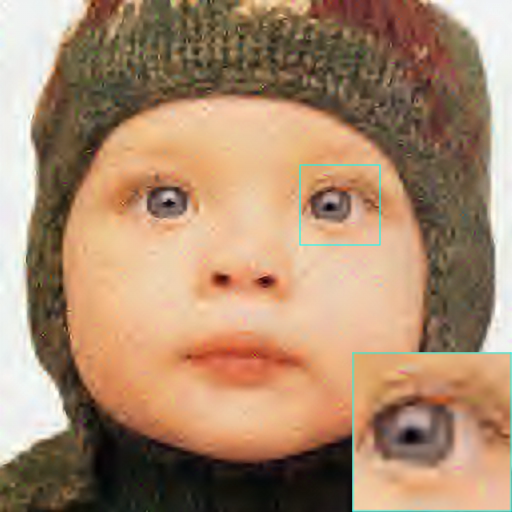
\includegraphics[width=\textwidth]{images/exp2.2/gaussian.png}
		\caption{Gaussian restored}
	\end{subfigure}
	\begin{subfigure}{0.24\textwidth}
		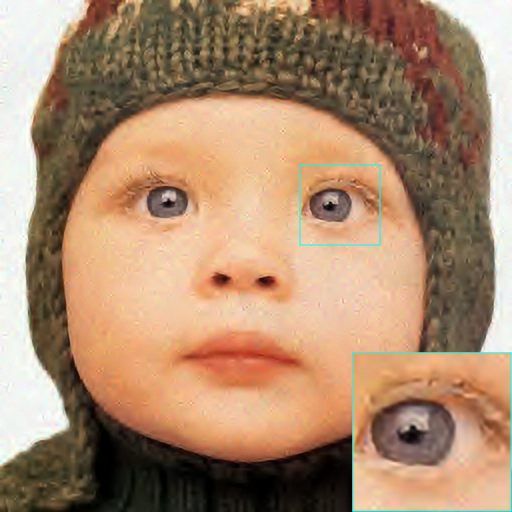
\includegraphics[width=\textwidth]{images/exp2.2/poisson.png}
		\caption{Poisson restored}
	\end{subfigure}
	\begin{subfigure}{0.24\textwidth}
		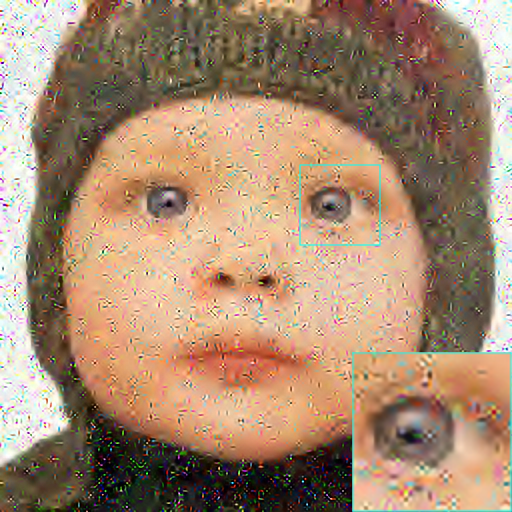
\includegraphics[width=\textwidth]{images/exp2.2/salt.png}
		\caption{S\&P restored}
	\end{subfigure}
	\begin{subfigure}{0.24\textwidth}
		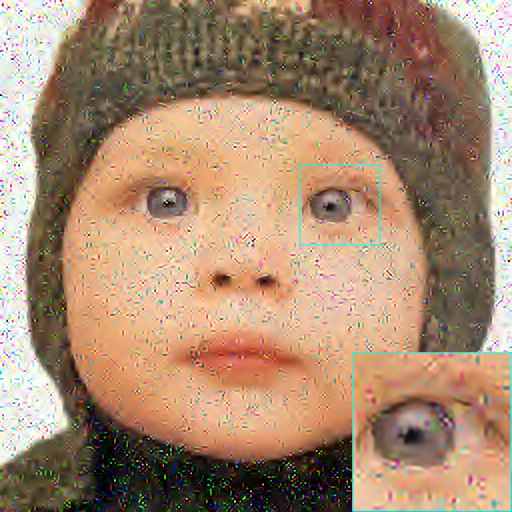
\includegraphics[width=\textwidth]{images/exp2.2/uniform.png}
		\caption{Uniform restored}
	\end{subfigure}
	\caption{Experiment 2.2: restoration using wavelet denoiser $+$ \gls{fsrcnn}}
	\label{fig:exp2.2}
\end{figure}

In the first instance, the wavelet denoiser is able to effectively reduce the noise for those types of noise that are additive or signal dependent, i.e., the Gaussian noise and the Poisson noise. However, the quality of the results is not as high as in the \gls{ircnn} results. 

On the other hand, if we take a look at the results of this combination on the images degraded by salt-and-pepper noise and uniform noise, we can observe that the wavelet algorithm cannot properly remove the noise, and therefore the final images present low-quality.

\subsection{Experiment 2.3}
In this experiment, we replace the wavelet denoiser of the previous experiment by a median filter. Therefore, we evaluate the results of applying a median filter + \gls{fsrcnn} on our set of \gls{lr} images. The metrics results of this experiment are presented in Table \ref{tab:experiment23}.

\begin{table}[]
	\centering
	\begin{tabular}{|l|l|r|r|r|r|}
		\hline
		\rowcolor[HTML]{EFEFEF} 
		\multicolumn{1}{|c|}{\cellcolor[HTML]{EFEFEF}\textbf{Noise}} & \textbf{Parameters} & \multicolumn{1}{c|}{\cellcolor[HTML]{EFEFEF}\textbf{Set5 \gls{psnr} (dB)}} & \multicolumn{1}{c|}{\cellcolor[HTML]{EFEFEF}\textbf{Set5 \gls{ssim}}} & \multicolumn{1}{c|}{\cellcolor[HTML]{EFEFEF}\textbf{Set14 \gls{psnr} (dB)}} & \multicolumn{1}{c|}{\cellcolor[HTML]{EFEFEF}\textbf{Set14 \gls{ssim}}} \\ \hline
		\rowcolor[HTML]{FFFFFF} 
		\cellcolor[HTML]{EFEFEF} & $\mu=0, \sigma=0.05$ & 25.9872 & 0.8739 & 23.9859 & 0.7578 \\
		\rowcolor[HTML]{EFEFEF} 
		\cellcolor[HTML]{EFEFEF} & $\mu=0, \sigma=0.10$ & 23.9557 & 0.8044 & 22.5017 & 0.6852 \\
		\rowcolor[HTML]{FFFFFF} 
		\multirow{-3}{*}{\cellcolor[HTML]{EFEFEF}Gaussian} & $\mu=0, \sigma=0.15$ & 22.0852 & 0.7334 & 20.9973 & 0.6142 \\
		\rowcolor[HTML]{EFEFEF} 
		Poisson & $peak=2^8$ & 26.2772 & 0.8925 & 24.1578 & 0.7690 \\
		\rowcolor[HTML]{FFFFFF} 
		\cellcolor[HTML]{EFEFEF} & $r=0.05$ & 26.8715 & 0.9165 & 24.5762 & 0.7983 \\
		\rowcolor[HTML]{EFEFEF} 
		\cellcolor[HTML]{EFEFEF} & $r=0.10$ & 26.0928 & 0.9069 & 24.0433 & 0.7888 \\
		\rowcolor[HTML]{FFFFFF} 
		\cellcolor[HTML]{EFEFEF} & $r=0.15$ & 25.1191 & 0.8942 & 23.3845 & 0.7751 \\
		\rowcolor[HTML]{EFEFEF} 
		\multirow{-4}{*}{\cellcolor[HTML]{EFEFEF}Salt-and-pepper} & $r=0.20$ & 23.8783 & 0.8750 & 22.5070 & 0.7551 \\
		\rowcolor[HTML]{FFFFFF} 
		\cellcolor[HTML]{EFEFEF} & $r=0.05$ & 26.9496 & 0.9171 & 24.6094 & 0.7979 \\
		\rowcolor[HTML]{EFEFEF} 
		\cellcolor[HTML]{EFEFEF} & $r=0.10$ & 26.2939 & 0.9076 & 24.2091 & 0.7878 \\
		\rowcolor[HTML]{FFFFFF} 
		\cellcolor[HTML]{EFEFEF} & $r=0.15$ & 25.5000 & 0.8921 & 23.6985 & 0.7726 \\
		\rowcolor[HTML]{EFEFEF} 
		\multirow{-4}{*}{\cellcolor[HTML]{EFEFEF}Uniform} & $r=0.20$ & 24.4354 & 0.8651 & 23.0633 & 0.7503 \\
		\rowcolor[HTML]{FFFFFF} 
		\textbf{All} &  & \textbf{25.2872} & \textbf{0.8732} & \textbf{23.4778} & \textbf{0.7543}\\\hline
	\end{tabular}
	\caption{\gls{psnr} and \gls{ssim} results for the Experiment 2.3}
	\label{tab:experiment23}
\end{table}

In the table, we can see that the average \gls{psnr} and \gls{ssim} results improve when we replace the wavelet denoiser by a median filter. However, even though the overall results and the results obtained on the images degraded with salt-and-pepper and uniform noise are better compared to the previous experiment, the wavelet denoiser overperforms the median filter on the images that presented with Gaussian and Poisson noise.

\begin{figure}
	\centering
	\begin{subfigure}{0.24\textwidth}
		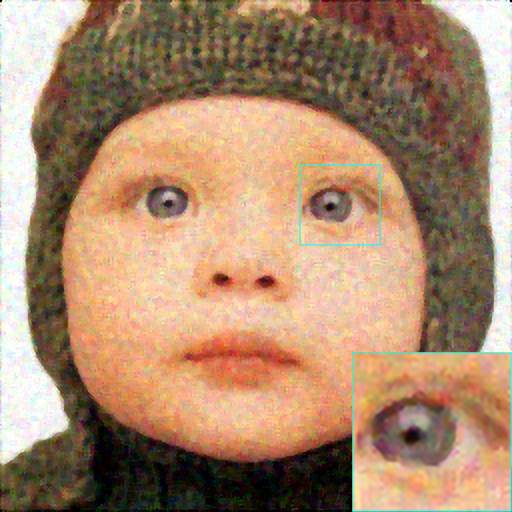
\includegraphics[width=\textwidth]{images/exp2.3/gaussian.png}
		\caption{Gaussian restored}
	\end{subfigure}
	\begin{subfigure}{0.24\textwidth}
		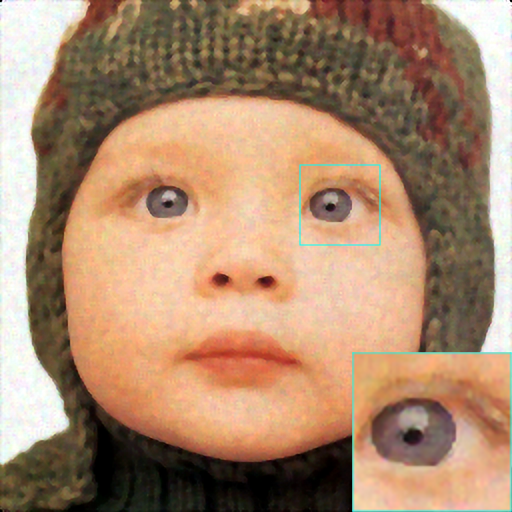
\includegraphics[width=\textwidth]{images/exp2.3/poisson.png}
		\caption{Poisson restored}
	\end{subfigure}
	\begin{subfigure}{0.24\textwidth}
		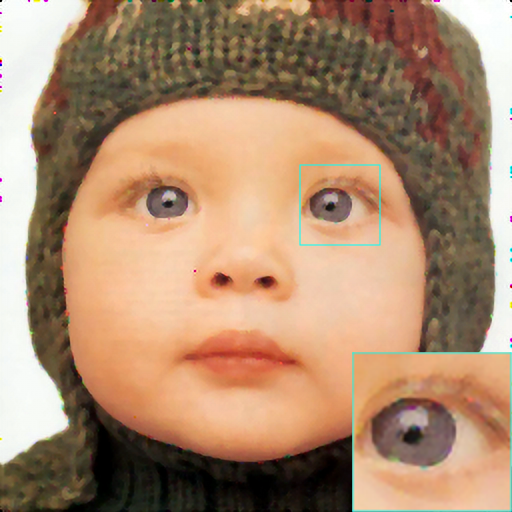
\includegraphics[width=\textwidth]{images/exp2.3/salt.png}
		\caption{S\&P restored}
	\end{subfigure}
	\begin{subfigure}{0.24\textwidth}
		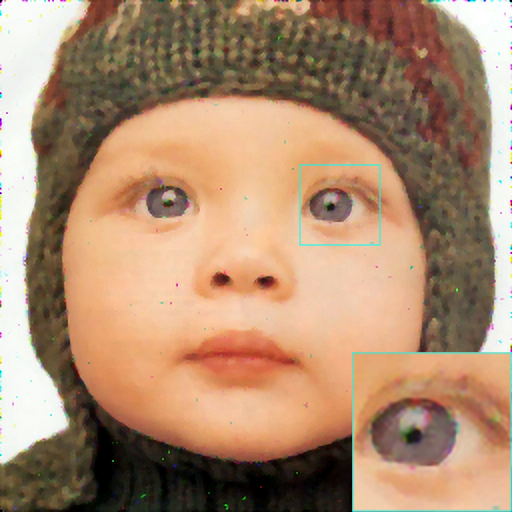
\includegraphics[width=\textwidth]{images/exp2.3/uniform.png}
		\caption{Uniform restored}
	\end{subfigure}
	\caption{Experiment 2.3: restoration using median filter $+$ \gls{fsrcnn}}
	\label{fig:exp2.3}
\end{figure}

This can also be observed in Figure \ref{fig:exp2.3}, in which we present the results of applying median filter $+$ \gls{fsrcnn} to the images of Figure \ref{fig:exp0}. The images that had Gaussian and Poisson noise still present a considerable amount of noise after the restoration. On the other hand, the images degraded with salt-and-pepper and uniform noise present a much lower amount of noise after applying the median filter. 

In any case, the performance obtained in Experiment 1.2. cannot be reached by using any of these traditional filters.



\subsection{Experiment 3.1}
\begin{table}[]
	\centering
	\begin{tabular}{|l|l|r|r|r|r|}
		\hline
		\rowcolor[HTML]{EFEFEF} 
		\multicolumn{1}{|c|}{\cellcolor[HTML]{EFEFEF}\textbf{Noise}} & \textbf{Parameters} & \multicolumn{1}{c|}{\cellcolor[HTML]{EFEFEF}\textbf{Set5 \gls{psnr} (dB)}} & \multicolumn{1}{c|}{\cellcolor[HTML]{EFEFEF}\textbf{Set5 \gls{ssim}}} & \multicolumn{1}{c|}{\cellcolor[HTML]{EFEFEF}\textbf{Set14 \gls{psnr} (dB)}} & \multicolumn{1}{c|}{\cellcolor[HTML]{EFEFEF}\textbf{Set14 \gls{ssim}}} \\ \hline
		\rowcolor[HTML]{FFFFFF} 
		\cellcolor[HTML]{EFEFEF} & $\mu=0, \sigma=0.05$ & 27.8760 & 0.9116 & 25.8165 & 0.8244 \\
		\rowcolor[HTML]{EFEFEF} 
		\cellcolor[HTML]{EFEFEF} & $\mu=0, \sigma=0.10$ & 25.2040 & 0.8553 & 23.7390 & 0.7520 \\
		\rowcolor[HTML]{FFFFFF} 
		\multirow{-3}{*}{\cellcolor[HTML]{EFEFEF}Gaussian} & $\mu=0, \sigma=0.15$ & 23.3125 & 0.8046 & 22.3406 & 0.7016 \\
		\rowcolor[HTML]{EFEFEF} 
		Poisson & $peak=2^8$ & 28.7267 & 0.9298 & 26.3338 & 0.8453 \\
		\rowcolor[HTML]{FFFFFF} 
		\cellcolor[HTML]{EFEFEF} & $r=0.05$ & 20.8489 & 0.7180 & 20.8049 & 0.6445 \\
		\rowcolor[HTML]{EFEFEF} 
		\cellcolor[HTML]{EFEFEF} & $r=0.10$ & 20.0257 & 0.6657 & 20.0924 & 0.5918 \\
		\rowcolor[HTML]{FFFFFF} 
		\cellcolor[HTML]{EFEFEF} & $r=0.15$ & 19.5516 & 0.6569 & 19.6361 & 0.5817 \\
		\rowcolor[HTML]{EFEFEF} 
		\multirow{-4}{*}{\cellcolor[HTML]{EFEFEF}Salt-and-pepper} & $r=0.20$ & 18.9040 & 0.6454 & 19.0571 & 0.5714 \\
		\rowcolor[HTML]{FFFFFF} 
		\cellcolor[HTML]{EFEFEF} & $r=0.05$ & 22.9494 & 0.7780 & 22.6777 & 0.7204 \\
		\rowcolor[HTML]{EFEFEF} 
		\cellcolor[HTML]{EFEFEF} & $r=0.10$ & 21.4818 & 0.7196 & 21.3892 & 0.6547 \\
		\rowcolor[HTML]{FFFFFF} 
		\cellcolor[HTML]{EFEFEF} & $r=0.15$ & 20.4685 & 0.6920 & 20.5239 & 0.6233 \\
		\rowcolor[HTML]{EFEFEF} 
		\multirow{-4}{*}{\cellcolor[HTML]{EFEFEF}Uniform} & $r=0.20$ & 19.5550 & 0.6708 & 19.7700 & 0.6028 \\
		\rowcolor[HTML]{FFFFFF} 
		\textbf{All} &  & \textbf{22.4087} & \textbf{0.7540} & \textbf{21.8485} & \textbf{0.6762}\\\hline
	\end{tabular}
	\caption{\gls{psnr} and \gls{ssim} results for the Experiment 3.1}
	\label{tab:experiment31}
\end{table}

\begin{figure}
	\centering
	\begin{subfigure}{0.24\textwidth}
		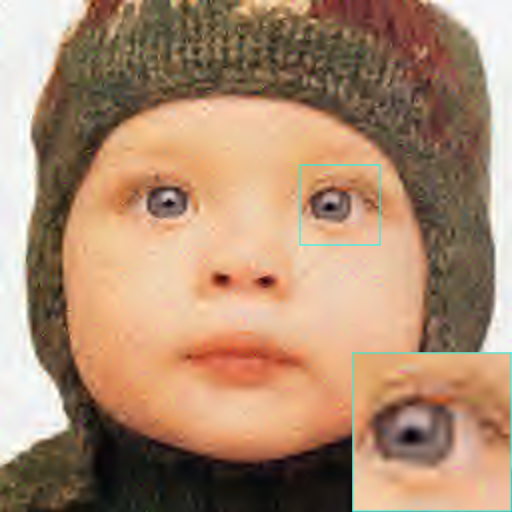
\includegraphics[width=\textwidth]{images/exp3.1/gaussian.png}
		\caption{Gaussian restored}
	\end{subfigure}
	\begin{subfigure}{0.24\textwidth}
		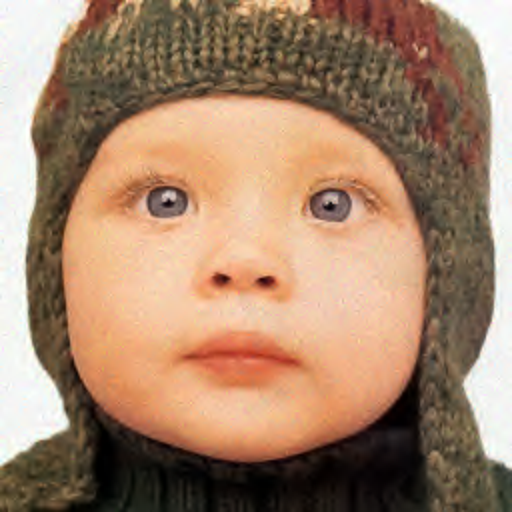
\includegraphics[width=\textwidth]{images/exp3.1/poisson.png}
		\caption{Poisson restored}
	\end{subfigure}
	\begin{subfigure}{0.24\textwidth}
		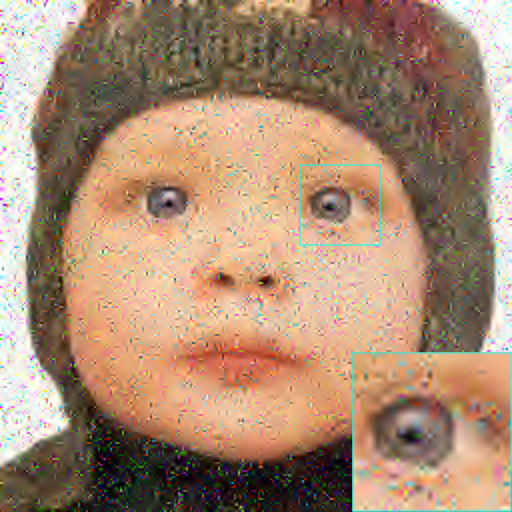
\includegraphics[width=\textwidth]{images/exp3.1/salt.png}
		\caption{S\&P restored}
	\end{subfigure}
	\begin{subfigure}{0.24\textwidth}
		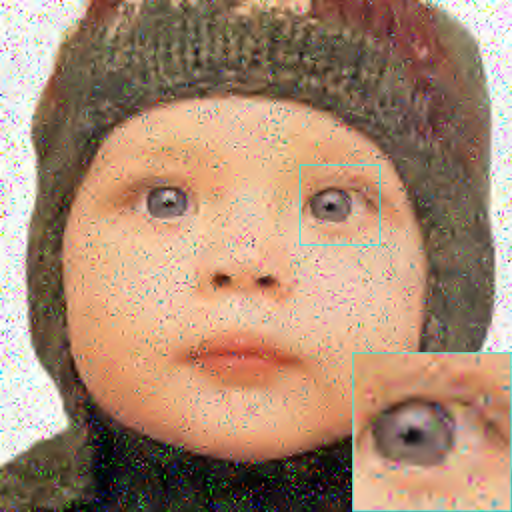
\includegraphics[width=\textwidth]{images/exp3.1/uniform.png}
		\caption{Uniform restored}
	\end{subfigure}
	\caption{Experiment 3.1: restoration using wavelet denoiser $+$ bicubic interpolation}
	\label{fig:exp3.1}
\end{figure}


\subsection{Experiment 3.2}
\begin{table}[]
	\centering
	\begin{tabular}{|l|l|r|r|r|r|}
		\hline
		\rowcolor[HTML]{EFEFEF} 
		\multicolumn{1}{|c|}{\cellcolor[HTML]{EFEFEF}\textbf{Noise}} & \textbf{Parameters} & \multicolumn{1}{c|}{\cellcolor[HTML]{EFEFEF}\textbf{Set5 \gls{psnr} (dB)}} & \multicolumn{1}{c|}{\cellcolor[HTML]{EFEFEF}\textbf{Set5 \gls{ssim}}} & \multicolumn{1}{c|}{\cellcolor[HTML]{EFEFEF}\textbf{Set14 \gls{psnr} (dB)}} & \multicolumn{1}{c|}{\cellcolor[HTML]{EFEFEF}\textbf{Set14 \gls{ssim}}} \\ \hline
		\rowcolor[HTML]{FFFFFF} 
		\cellcolor[HTML]{EFEFEF} & $\mu=0, \sigma=0.05$ & 26.2755 & 0.8812 & 24.2264 & 0.7663 \\
		\rowcolor[HTML]{EFEFEF} 
		\cellcolor[HTML]{EFEFEF} & $\mu=0, \sigma=0.10$ & 24.2735 & 0.8134 & 22.8012 & 0.6979 \\
		\rowcolor[HTML]{FFFFFF} 
		\multirow{-3}{*}{\cellcolor[HTML]{EFEFEF}Gaussian} & $\mu=0, \sigma=0.15$ & 22.4366 & 0.7452 & 21.3403 & 0.6299 \\
		\rowcolor[HTML]{EFEFEF} 
		Poisson & $peak=2^8$ & 26.6459 & 0.9059 & 24.4262 & 0.7795 \\
		\rowcolor[HTML]{FFFFFF} 
		\cellcolor[HTML]{EFEFEF} & $r=0.05$ & 27.1121 & 0.9209 & 24.7449 & 0.8034 \\
		\rowcolor[HTML]{EFEFEF} 
		\cellcolor[HTML]{EFEFEF} & $r=0.10$ & 26.3782 & 0.9123 & 24.2646 & 0.7950 \\
		\rowcolor[HTML]{FFFFFF} 
		\cellcolor[HTML]{EFEFEF} & $r=0.15$ & 25.4810 & 0.9009 & 23.6647 & 0.7829 \\
		\rowcolor[HTML]{EFEFEF} 
		\multirow{-4}{*}{\cellcolor[HTML]{EFEFEF}Salt-and-pepper} & $r=0.20$ & 24.3109 & 0.8836 & 22.8559 & 0.7650 \\
		\rowcolor[HTML]{FFFFFF} 
		\cellcolor[HTML]{EFEFEF} & $r=0.05$ & 27.1583 & 0.9208 & 24.7666 & 0.8026 \\
		\rowcolor[HTML]{EFEFEF} 
		\cellcolor[HTML]{EFEFEF} & $r=0.10$ & 26.5295 & 0.9116 & 24.3931 & 0.7933 \\
		\rowcolor[HTML]{FFFFFF} 
		\cellcolor[HTML]{EFEFEF} & $r=0.15$ & 25.7746 & 0.8967 & 23.9241 & 0.7793 \\
		\rowcolor[HTML]{EFEFEF} 
		\multirow{-4}{*}{\cellcolor[HTML]{EFEFEF}Uniform} & $r=0.20$ & 24.7671 & 0.8715 & 23.3377 & 0.7590 \\
		\rowcolor[HTML]{FFFFFF} 
		\textbf{All} &  & \textbf{25.5953} & \textbf{0.8803} & \textbf{23.7288} & \textbf{0.7628}\\\hline
	\end{tabular}
	\caption{\gls{psnr} and \gls{ssim} results for the Experiment 3.2}
	\label{tab:experiment32}
\end{table}


\begin{figure}
	\centering
	\begin{subfigure}{0.24\textwidth}
		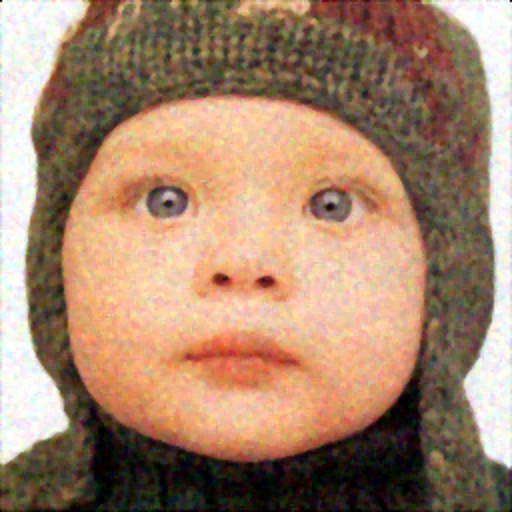
\includegraphics[width=\textwidth]{images/exp3.2/gaussian.png}
		\caption{Gaussian restored}
	\end{subfigure}
	\begin{subfigure}{0.24\textwidth}
		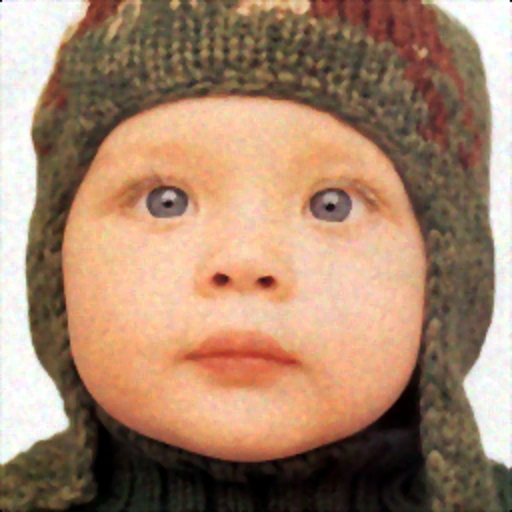
\includegraphics[width=\textwidth]{images/exp3.2/poisson.png}
		\caption{Poisson restored}
	\end{subfigure}
	\begin{subfigure}{0.24\textwidth}
		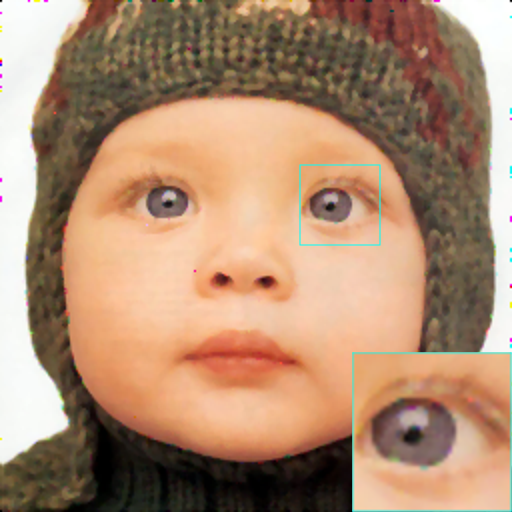
\includegraphics[width=\textwidth]{images/exp3.2/salt.png}
		\caption{S\&P restored}
	\end{subfigure}
	\begin{subfigure}{0.24\textwidth}
		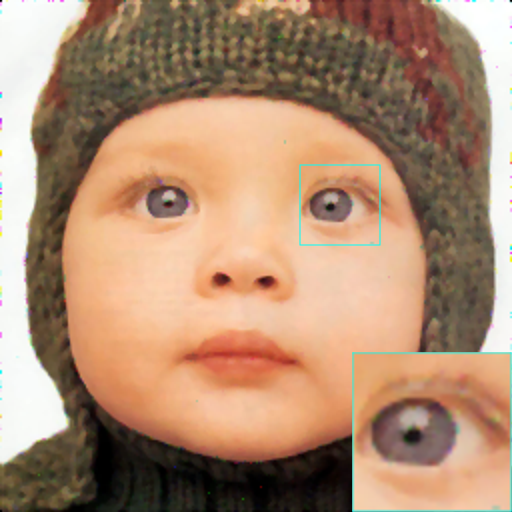
\includegraphics[width=\textwidth]{images/exp3.2/uniform.png}
		\caption{Uniform restored}
	\end{subfigure}
	\caption{Experiment 3.2: restoration using median filter $+$ bicubic interpolation}
	\label{fig:exp3.2}
\end{figure}

\subsection{Results summary}
